% !TEX root = DesignDoc.tex

\chapter{ROS Architecture}
\label{chap:rosarch}

The SMP and Mecanum robots have identical ROS architecture with the exception of the drivers used to control the motor controllers. With a more complex robot, this section would be considerably longer, but there isn't actually a whole lot going on to just make a robot drive under RC control.

\section{Nodes}

The following ROS nodes are running on the SMPs:

\begin{itemize}
\item{joy\_to\_twist}
\item{skid\_drive\_controller}
\item{roboteq\_nxtgen\_controller}
\end{itemize}

The following ROS nodes are running on Mecanum:

\begin{itemize}
\item{joy\_to\_twist}
\item{mecanum\_drive}
\item{orion\_roboclaw\_driver}
\end{itemize}

\section{rqtplot}

\begin{figure}[h]
\centering
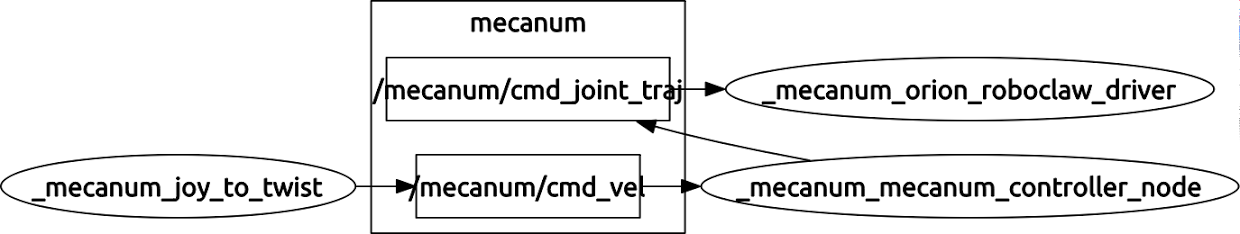
\includegraphics[width=\textwidth]{rqtplotmecanum.png}
\label{fig:rqtplotmecanum}
\caption{Mecanum rqtplot}
\end{figure}

I'll be adding one for the SMPs when I get a chance to do some remote work through someone at the lab. The one for mecanum isn't quite what I expected to see, so I'll have to look in to that as well.

\section{Other Packages}

The SMPs also require the smp\_bringup package with contains the default launch file. Mecanum has no corresponding package, but does require a very similar launch file which calls for the different drive and motor control nodes.

\section{Other Files}

The SMP launch file, udev rules, and smp\_bringup.service file are included with this document. The Mecanum variants will also be included once I get them from Dan and Joe, who currently have the robot.
